\begin{figure}[h]
    \centering
    %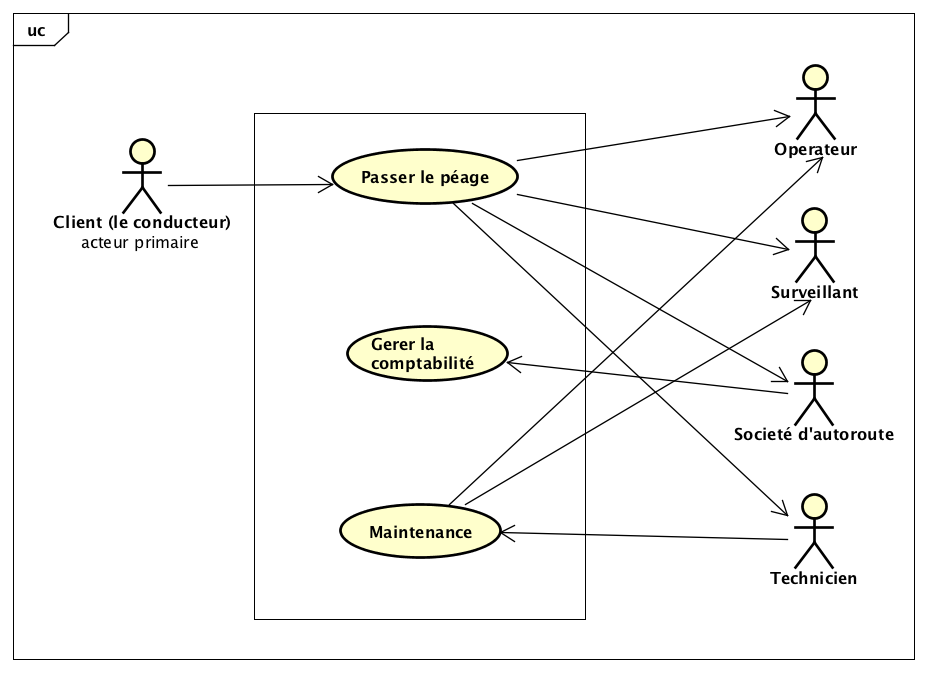
\includegraphics[scale=0.50]{02_Desenvolvimento/TD2/images/hautNiveau.png}
    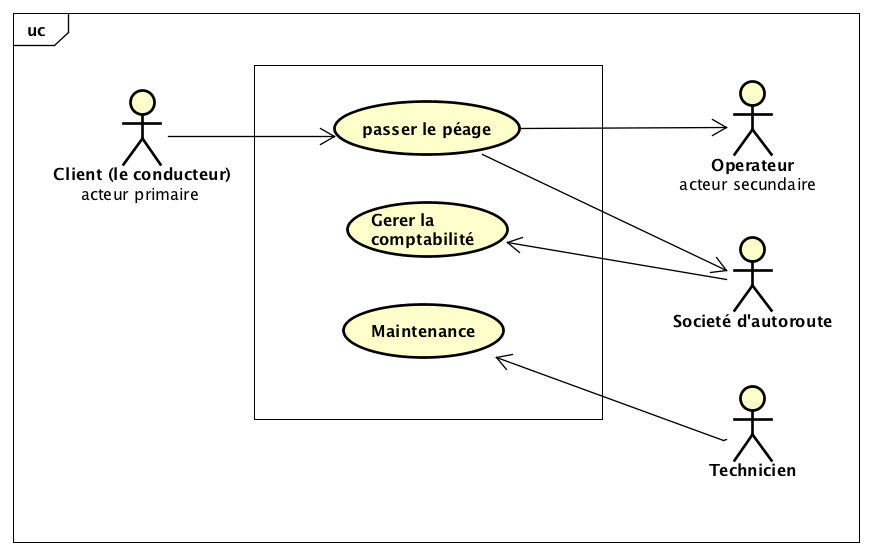
\includegraphics[scale=0.50]{02_Desenvolvimento/TD2/images/UseCaseDiagram.png}
    \caption{Diagramme de haut niveau - Péage}
    \label{fig:hautNiveau}
\end{figure}

\textbf{Cockburn Bref:} Passer le péage\\
Le client (le conducteur) opte pour une voie d’autoroute selon son type de véhicule et le moyen de paiement. La borne détecte et valide le véhicule. Le conducteur effectue le paiement selon le type de borne qu’il a choisi (avec une carte d’abonnement, carte de crédit, monnaie, monnaie à un opérateur humain, etc). Le système gère l’ouverture de la barrière une fois le montant payé ou la carte d’abonnement présenté. Si la barrière ne s’ouvre pas ou si la borne détecte un véhicule non autorisé, alors un technicien ou un opérateur doit venir régler l’incident survenu. Si une borne automatique n'a plus de mannaie, donc il faut lever une alarme vers l'ordinateur du poste de surveillance. C'est le même traitement le déclenchement des mouvements de barrières, des affichages des panneaux indicatifs de l'ouverture au de la fermeture de la voie, la sychronisation feu et aval, etc.

\textbf{Cockburn Bref:} Gerer la comptabilité \\
Le système doit assurer la comptabilité générale de l’ensemble des bornes. Chaque levée de barrière est enregistré. Les cartes d’abonnement et les compte des abonnés sont gérés par la société d’autoroute de façon instantanée, chaque passage est enregistré. Les opérations par cartes bleues sont gérées en fin de journée. Les bornes détectent les fausses pièces et les cartes volées.

\textbf{Cockburn Bref:} Maintenance  \\
Le technicien permet de gérer toutes les cas, incidents, qui nécessitent une intervention humaine, lorsque qu’une barrière doit être ouverte ou fermée manuellement, lorsqu’un usager se retrouve coincé à la barrière de péage ou lorsqu’une borne a besoin de réglage ou de réparation (comme remettre de la monnaie).